\section{Implementation, validation, and measured effects}
\label{sec:experiments}

\subsection{Integration choices}
The archive contains an integrated \code{fastunknot} version 0.3.0 in
\code{fast/}. The unchanged pinned source is under \code{reference/fast/};
the supplied patch applies the implementation changes to the original
repository path. No remote branch or commit is modified by this deliverable.

The structural certificate runs before the legacy reduction and filtering
pipeline. This placement gives linear recognition on homogeneous input
diagrams without first allocating an Alexander matrix. It also imposes an
extra traversal when inconclusive, including on a diagram that elementary
reduction would immediately settle. The option \code{use\_seifert=False},
or \code{--no-seifert} on the command line, restores the previous stage
ordering. This is a measured tradeoff, not a universal speedup claim.

The ordinary scanner remains the default fallback. The new selectable
backends are \code{shared}, \code{saturated}, and \code{euler}:
\begin{center}\small
\begin{tabularx}{\textwidth}{@{}lYY@{}}
\toprule
Backend & Information retained & Returned homology evidence\\
\midrule
\code{standard} & Original explicit representatives & Exact ranks and raw
homological-degree counts\\
\code{shared} & One representative per exact key; $\N[z]$ weights & The
same exact ranks and degree counts\\
\code{saturated} & Relative template degrees and $S_3$ weights & Final
\code{rank\_capped}, with cap three\\
\code{euler} & Saturated sharing plus bounded exact suffix evaluation &
An early \code{rank\_lower\_bound\_capped}, or a final
\code{rank\_capped}\\
\bottomrule
\end{tabularx}
\end{center}
The new backends currently use the existing bit algebra and minimum-fill
pivot policy. Incompatible requests for the set algebra, alternative pivots,
tail contraction, or multi-process scan races are rejected explicitly.
They are not silently ignored. The exact-rank command also accepts
\code{--shared}. The low-level interfaces retain the valid classical
one-component input promise described in Section~\ref{sec:model}.

In shared modes, \code{max\_objects} limits actual allocated representative
objects before elimination. It does not limit the number of virtual copies.
Time limits are cooperative rather than hard process deadlines, as in the
baseline. Object or time exhaustion gives \UNKNOWN. Exceeding the optional
Euler-state budget only disables that inference and continues the exact
decision scan. Early Euler evidence is a certified lower bound and is never
labeled as a completed exact rank. In saturated mode, statistics concerning
expanded multiplicity are named as lower bounds.

\subsection{Validation design}
The final test log accompanies the code. The suite has 69 test methods:
41 inherited methods, six structural-certificate methods, nine component
methods, eight Euler methods, and five public integration methods. The two
inherited pipeline test modules explicitly disable the new structural stage
when asserting old method names; new tests exercise the new default. This
retains the meaning of the baseline regression tests rather than changing
their expected intermediate methods wholesale.

The checks address independent failure mechanisms:
\begin{itemize}
\item Structural data are compared with closed-braid formulas on 160
fixed-seed random closures, including mirrors, row half-turns, crossing
permutations, and edge relabelings. Issued certificates are compared with
exact Khovanov recognition on 60 short random closures. An independent
orientation reconstruction and union--find verifier replays certificates;
forged fields and the misleading zero Rasmussen interval are tested.
\item Component sharing is compared with the original scanner on 200
fixed-seed random valid closures, half with arbitrary random crossing orders.
The suite checks $d^2=0$ after every scan stage and includes comparisons with
the independently represented generic set algebra. Tests cover exact-key
equality, integer rather than parity multiplicities, degree shifts,
mirrors, torus examples, and resource limits.
\item Suffix Euler values are compared with explicit continuation using
the generic algebra on 40 random prefixes. Fifty random arbitrary-order
diagrams check monotonicity of the bound and equality with the rank at final
closure. Additional tests cover signed cancellation, mirror conventions,
safe budget exhaustion, and a 1,201-crossing order handled without recursion.
\item Integration checks compare the default pipeline with the legacy
pipeline on 100 random closures, exercise all four backends, replay default
certificates, and check JSON fields and command-line rejection of
incompatible options.
\end{itemize}
The finite family check in \code{benchmarks/defect\_one\_family.py}
independently tests the symbolic formulas of
Section~\ref{sec:reduced-defect-one} for all $2\le k\le100$: 99 diagrams
through 202 crossings. This verifies the implementation of the family;
the proof for arbitrary $k$ is the symbolic argument in the article.
These tests support an exact implementation but are not a machine-checked
proof of the entire inherited cobordism algebra or of the external
topological theorems.

\subsection{Structural-stage experiment}
Twenty cases were measured in nine randomized, interleaved rounds. Each
round included the baseline arm $A$, the new structural-first arm $B$, and
two identical baseline control arms. Every invocation received a fresh,
uncached \emph{already validated} PD diagram. The measured boundary is the
recognition function; parsing, validation, imports, file I/O, and result
serialization are excluded symmetrically. This is the boundary at which
the front end is inserted. Both implementations share the same unchanged
fallback pipeline.

For each case, paired speedup is the geometric mean of the nine $A/B$
wall-time ratios. The intervals below are 95\% percentile bootstrap
intervals of the paired mean log ratio, with 3,000 fixed-seed resamples.
They describe variation in this shared-host experiment, not a universal
hardware-independent confidence statement. The median times and paired
ratio are different summaries and need not divide to the same value.

\begin{table}[htbp]
\centering\small
\begin{tabular}{@{}lrrrr@{}}
\toprule
Family & $n$ & Median $A$ (ms) & Median $B$ (ms) & Paired speedup\\
\midrule
$\widehat{(\sigma_1\sigma_2^{-1})^{500}}$ & 1,000 & 62.1 & 2.14 & 28.75\\
$\widehat{(\sigma_1\sigma_2)^{500}}$ & 1,000 & 60.6 & 2.05 & 25.97\\
$\widehat{(\sigma_1\sigma_2\sigma_3\sigma_4)^{251}}$ & 1,004 & 129.8 & 2.02 & 53.94\\
\bottomrule
\end{tabular}
\caption{Recognition-function measurements on homogeneous families. The
paired speedup intervals are respectively $[25.59,31.98]$,
$[20.97,32.83]$, and $[44.86,63.75]$. All rows are knots.}
\label{tab:structural}
\end{table}

The baseline decided these cases with its modular Alexander stage. The new
certificate avoids that stage, including its dense matrix allocation.
The mathematical improvement is an $O(n)$ word-operation decision for this
class; the timing data illustrate that improvement but do not estimate the
exponent of the general recognizer. The usual $O(n^3)$ field-operation
bound on dense elimination is an upper bound, and these timings do not
claim that the chosen braid family attains it.

A second complete experiment pinned execution to CPU 8, disabled cyclic
garbage collection, and used longer timing batches. Its paired speedups on
the same three large cases were 27.86, 28.88, and 44.13. The large-family
advantage therefore persisted under this changed measurement protocol.
The original and repeated raw observations are both included.

Inconclusive controls expose the cost of the additional pass:
\begin{center}\small
\begin{tabular}{@{}lrr@{}}
\toprule
Control & Original paired $A/B$ & Repeated paired $A/B$\\
\midrule
Conway knot & 0.861 & 1.003\\
Kinoshita--Terasaka knot & 0.918 & 0.883\\
Eight-crossing hard unknot & 0.770 & 0.953\\
Six-crossing reducible grid unknot & 0.478 & 0.470\\
\bottomrule
\end{tabular}
\end{center}
Ratios below one favor the baseline. The tiny grid example rises from about
22 microseconds to 49--52 microseconds. Identical-arm controls show
substantial noise on tiny cases, even after pinning; moderate percentage
changes on the other controls should not be read as precise stable effects.
The substantial large-family gains and the approximately 30-microsecond
cost on the immediately reducible grid input are the robust conclusions.

\subsection{Component-sharing experiment}
The scanner experiment deliberately disables geometric factorization and
all recognition filters. It measures the algebraic backend itself. Seven
shuffled rounds per case contain two original-scanner arms, full sharing,
and saturated sharing. The recorded crossing order and output ranks are
checked. Define the deterministic work counter as
\[
 W=\code{entries}+\code{compositions}.
\]
This counter omits Python bookkeeping, key construction, multiplicity
updates, and Euler work. It is useful for interpreting the algebraic change;
it is not a machine-independent running-time bound.

\begin{table}[htbp]
\centering\small
\begin{tabular}{@{}lrrrrr@{}}
\toprule
Input & $W$ old & $W$ shared & Peak old & Peak shared & Full time ratio\\
\midrule
Conway & 1,609 & 1,605 & 246 & 246 & 1.220\\
$T(3,5)$ & 397 & 397 & 54 & 54 & 1.220\\
Stress braid, 36 crossings & 275,165 & 285,445 & 17,694 & 17,694 & 1.312\\
Two Conway summands & 58,844 & 6,875 & 8,118 & 975 & 0.244\\
Three Conway summands & 1,952,418 & 12,437 & 267,894 & 975 & 0.00735\\
\bottomrule
\end{tabular}
\caption{Raw scanner comparison. Peak means objects allocated before
elimination. Time ratio is median paired new/old, using the geometric mean
of the two old arms within each round. Smaller ratios favor sharing.}
\label{tab:sharing}
\end{table}

Saturated-sharing time ratios on the same rows are 1.188, 1.145, 1.284,
0.253, and 0.00793. The identical-arm ratios range approximately from 0.85
to 1.34 across these runs. The repeated-sum savings greatly exceed that
variation. On the prime controls, sharing does not reveal a useful
decomposition until very late and adds overhead. Different pivot ordering
after representative normalization can also change algebraic work; the
stress example's work increases slightly. Hence sharing is an optional
backend, with no claim that it dominates the existing scanner.

Eight Conway summands provide a larger representation check. The exact
unreduced rank is
\[
 2\cdot33^8=2{,}812{,}817{,}236{,}482.
\]
The sharing run uses at most 975 objects before elimination and 240
representative objects after sharing. The full mode performs 16,162
multiplicity updates; saturation reduces that counter to 377. A single
diagnostic run completed in about 0.095 seconds in full mode and 0.088
seconds in saturated mode. These single timings are not a paired speedup
estimate; the exact rank, allocation counts, and update counts are the
reproducible evidence of compression.

\textbf{This repeated-sum experiment does not establish an end-to-end
recognition improvement.} The pinned recognizer already splits visible
connected sums geometrically and can reject one nontrivial factor. It also
has polynomial filters that settle many of the prime controls. The experiment
establishes that literal repeated homological summands can be processed
without expanding their multiplicities. Its contribution to general
recognition remains dependent on finding useful analogous structure in
the filter-resistant prime residual class.

\begin{figure}[htbp]
\centering
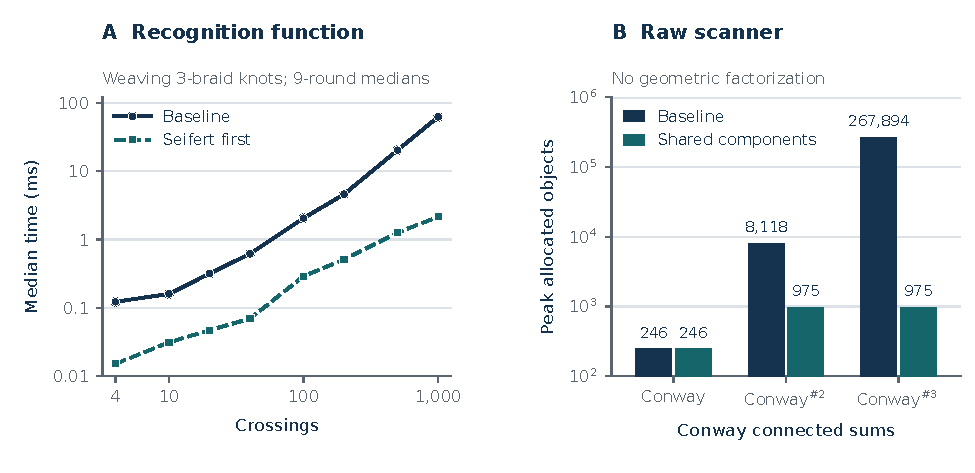
\includegraphics[width=\textwidth]{figures/performance_summary.pdf}
\caption{Two improvements with different measurement boundaries.
(A) Median recognition-function times on weaving three-strand knots in the
original structural experiment, nine rounds per input; parsing and validation
are excluded. Logarithmic axes and connecting segments show measurements,
with no fitted exponent. (B) Recorded maximum objects before elimination
in the raw baseline and exact shared scanners on one, two, and three Conway
summands, with geometric factorization disabled. These are scanner-object
counts, not process-memory measurements.}
\label{fig:performance}
\end{figure}

\subsection{Early Euler certificates}
The exact continuation recorder gives the following operation counts:
\begin{center}\small
\begin{tabular}{@{}lrrrr@{}}
\toprule
Input & Decision stage & Euler states & Scan $W$ at decision & Full shared $W$\\
\midrule
Two Conway summands & $11/22$ & 34 & 5,252 & 6,875\\
Three Conway summands & $11/33$ & 76 & 5,407 & 12,437\\
Eight Conway summands & $11/88$ & 286 & 5,252 & 39,317\\
\bottomrule
\end{tabular}
\end{center}
In each certificate the retained template has exact completed Euler
characteristic $+2$ and saturated multiplicity three. The resulting
nonnegative rank lower bound is capped at three and already exceeds the
unknot threshold. A one-state Euler budget on the eight-summand input
exhausts safely and completes the ordinary saturated scan at stage 88.

The Conway knot, stress braid, and hard-unknot controls trigger no Euler
states because they do not split early. The $T(3,5)$ example uses three
Euler states but yields no early verdict. It is a useful reminder that
nontrivial homology can have zero Euler characteristic within a summand.
The table counts Euler states separately: omitting their cost from $W$
must not be interpreted as omitting it from running time. No general
Euler-engine speedup is claimed from these diagnostic observations.

\subsection{What the evidence does and does not establish}
The structural front end changes the asymptotic cost of recognition on a
large, mathematically defined diagram class. The shared representations
remove an explicit multiplicity barrier and satisfy the finite-type theorem.
The Euler extension can use surviving summands as exact early witnesses.
All three are implemented and reproducibly tested.

The observed examples do not bound the sizes of future connected components,
prove a small frontier for arbitrary inputs, or certify that random tests
represent hard unknot diagrams. No fitted empirical exponent substitutes
for those missing structural statements. The default remains a complete
recognizer with an exponential worst-case upper bound, with \UNKNOWN\ under
optional resource ceilings. The following research programme addresses the
missing general theorem directly.
